% voorbeeld.tex
%
\documentclass[11pt,a4paper]{amsart}
\usepackage{amsmath,amssymb,amsthm}
\usepackage[utf8]{inputenc}
\usepackage[dutch]{babel}
\usepackage{enumitem}
\usepackage{graphicx}
%
\newtheorem{stelling}{Stelling}
%
\DeclareMathOperator{\opp}{opp}
%
\title{Een \LaTeX-voorbeeld}
\author{Kris Coolsaet}
%
\begin{document}
\maketitle
\section{Stelling van Pythagoras}

De \textbf{stelling van Pythagoras} is een wiskundige stelling die haar naam 
dankt aan de Griekse wiskundige Pythagoras. `Zijn' stelling was overigens 
alleen maar nieuw voor de Grieken. In Soemerië was het resultaat al veel langer 
bekend, en ook in Babylonië en het oude Egypte werd ze al eerder toegepast (met 
name de verhouding \(a=3\), \(b=4\), \(c=5\) werd al vroeg gebruikt om rechte hoeken uit te 
meten, zoals dat tot op de dag van vandaag door sommigen nog wordt gedaan). 

Echter, belangrijker dan de kennis van de stelling om haar enkel toe te passen, 
is het leveren van een bewijs. Wat dat betreft waren de Grieken (Pythagoras of 
een van zijn leerlingen) wel de eersten. Zij wisten niet alleen dat de stelling 
waar was, maar konden ook in algemene termen (abstracties) aantonen waarom zij 
waar was.

De stelling van Pythagoras geeft een verband tussen de lengten van de zijden 
van een rechthoekige driehoek. In woorden luidt de stelling:

\begin{stelling}[Propositie I.47 uit de \emph{Elementen van Euclides}]
\label{st-pythagoras}
In een rechthoekige driehoek is de som van de kwadraten van de lengtes van de 
rechthoekszijden gelijk aan het kwadraat van de lengte van de schuine zijde.
\end{stelling}

Noemen we de lengten van rechthoekszijden (de zijden die aan de hoek van 
90\({}^\circ\) 
liggen) \(a\) en \(b\), en de lengte van de schuine zijde (de zijde die niet 
aan de rechte hoek grenst, ook wel \emph{hypotenusa} genoemd) \(c\), dan is de 
bekende wiskundige vorm van de stelling:
\begin{equation}
\label{eq-pythagoras}
a^2 + b^2 = c^2.
\end{equation}

Stelling \ref{st-pythagoras} is equivalent met het \emph{parallellenpostulaat} 
\cite{Brodie}. 
Daarom 
geldt de stelling van Pythagoras niet in de niet-euclidische meetkunde.


\subsection{Voorbeeld}

Een rechthoekige driehoek heeft rechthoekszijden met lengten \(a=3\) en 
\(b=4\). De 
schuine zijde heeft de lengte \(c\). Wegens (\ref{eq-pythagoras}) geldt 
nu:
\[ c^2=a^2 + b^2 = 3^2+4^2=9+16=25. \]
Omdat de lengte \(c\) niet negatief kan zijn, is
\[c=\sqrt{25}=5.\]
Als van dezelfde driehoek de lengten \(b=4\) en \(c=5\) gegeven zijn, volgt de 
lengte \(a\) 
van de overgebleven zijde uit:
\[a^2=c^2 - b^2 = 5^2-4^2=25-16=9.\]
Omdat de lengte \(a\) niet negatief kan zijn, is
\[a=\sqrt {9}=3\]

\subsection{Bewijzen}
\paragraph{Bewijs met opdelen vierkant}
Een van de meer eenvoudige bewijzen deelt een vierkant met zijde \(a+b\) op 
twee 
manieren in.
\begin{center}
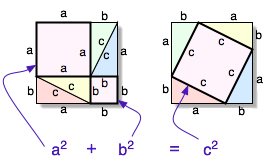
\includegraphics{Pythagorean_proof.png}
\end{center}

\begin{proof}
In de linkerfiguur is het vierkant opgebouwd uit een vierkant met 
zijde a, een vierkant met zijde \(b\), en 4 rechthoekige driehoeken waar we mee 
begonnen. De rechterfiguur is een vierkant opgebouwd uit een vierkant met zijde 
\(c\), en wederom de \(4\) rechthoekige driehoeken.

In beide figuren zien we een vierkant met zijde \(a+b\), dus beide vierkanten 
hebben dezelfde oppervlakte. Laten we nu zowel links als rechts de vier 
rechthoekige driehoeken weg, dan hebben de figuren die je overhoudt nog steeds 
dezelfde oppervlakte. Maar links houd je een vierkant met zijde \(a\), en een 
vierkant met zijde \(b\) over, met samen een oppervlakte van \(a^2+b^2\). 
Rechts houd je 
een vierkant met zijde \(c\) over, met een oppervlakte van \(c^2\). Hieruit 
volgt de 
stelling.
\end{proof}

Voor mensen die van meer algebraïsche bewijzen houden, ziet het bewijs er als 
volgt uit.
\begin{proof}
Telkens zijn er een korte en een lange zijde in elkaars verlengde 
geplaatst. De lengte en breedte van de zijden van het vierkant zijn \((a+b)\), 
dus 
de oppervlakte van het grote vierkant is \((a+b)^2\).

De oppervlakte is ook gelijk aan de som van de vier driehoeken 
\((4\times\frac12 ab)\) plus 
de oppervlakte van het binnenste vierkant, dat oppervlakte \(c^2\) heeft.

Dus
\[ (a+b)^2 = 2ab + c^2.\]
Uitwerken van het kwadraat links geeft:
\[a^2 + 2ab + b^2 = 2ab + c^2.\]
Dus
\[
a^2+b^2 = c^2.\qedhere
\]
\end{proof}

\paragraph{Bewijs met gelijkvormigheid}
Een ander inzichtelijk bewijs maakt gebruik van een hulplijn. Hiertoe dient de 
hoogtelijn vanuit de rechte hoek \(C\), die zijde \(AB\) snijdt in het punt 
\(D\).
\begin{center}
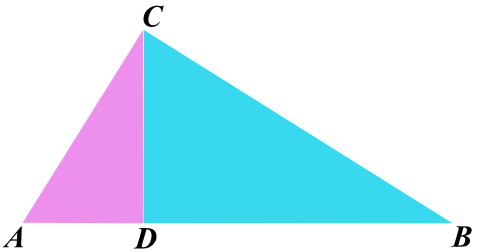
\includegraphics[scale=0.35]{P_triangle.png}
\end{center}
\begin{proof}
Het is nu snel in te zien dat driehoek \(ACD\) gelijkvormig is aan driehoek 
\(ABC\). 
Immers, de hoeken bij \(A\) zijn dezelfde, en beide driehoeken hebben ook een 
rechte hoek, bij \(C\) resp. \(D\).

Op dezelfde manier zien we dat driehoek \(CBD\) gelijkvormig is aan driehoek 
\(ABC\). 

We hebben dus drie gelijkvormige driehoeken. Kijken we naar de verhoudingen van 
de lengtes van de zijden van de driehoeken, dan zien we dat die gelijk zijn aan 
\(a:b:c\), immers precies de schuine zijden van de drie driehoeken. Dat 
betekent 
dat de oppervlaktes van de driehoeken zich verhouden als \(a^2:b^2:c^2\), de 
kwadraten 
van de verhoudingen van de zijden. Omdat duidelijk is dat \(\opp(CBD) + 
\opp(ACD) 
= 
\opp(ABC)\), geldt kennelijk voor een bepaald getal \(k\) dat 
\(ka^2+kb^2=kc^2\). En Stelling \ref{st-pythagoras} volgt nu door deling door 
\(k\).
\end{proof}

\subsection{Pythagorese drietallen}
De kleinste positieve gehele getallen die aan relatie (\ref{eq-pythagoras}) 
voldoen zijn 3,4,5, immers \(3^2 + 4^2 = 5^2\). Zo'n drietal heet een 
\emph{Pythagorees drietal}. Uiteraard voldoet ook elk geheel veelvoud hiervan, 
zoals 
\(6^2 + 8^2 = 10^2\). Dit is eenvoudig als volgt in te zien: als \((a,b,c)\) 
een 
Pythagorees drietal is, dan geldt dat \(a^2 + b^2 = c^2\). Daaruit volgt dat 
\(k^2(a^2 + 
b^2) = k^2c^2\), ofwel \(k^2a^2 + k^2b^2 = k^2c^2\), dus is \((ka,kb,kc)\) ook 
een Pythagorees 
drietal.

Ook als men de veelvouden van een drietal niet meetelt, dus als de drie 
getallen relatief priem zijn, zijn er oneindig veel combinaties van positieve 
gehele getallen die aan (\ref{eq-pythagoras}) voldoen. (5,12,13) is een 
andere bekende combinatie.

De algemene vorm voor Pythagorese drietallen die relatief priem zijn, is:
\[t^2-s^2,\quad 2ts \quad \text{en}\quad  t^2+s^2,\]
waarin t en s positieve gehele getallen zijn, relatief priem en met \(t>s\).

Er geldt immers:

\[(t^2-s^2)^2+(2ts)^2 = (t^2+s^2)^2.\]
Voor \(t=2\) en \(s=1\) krijgen we de relatie: \(3^2 + 4^2 = 5^2\).

\subsection{Goniometrische grondformule}
Uit de stelling van Pythagoras volgt eveneens de grondformule van de 
goniometrie. Voor een rechthoekige driehoek met schuine zijde gelijk aan 1 
geldt namelijk:

\[\sin^2\alpha+\cos^2\alpha=1\]
\subsection{Euclidische afstand}

De \emph{afstandsformule} in het cartesisch coördinatenstelsel is van de 
stelling van 
Pythagoras afgeleid. De euclidische afstand 
van een punt \((x_1, y_1)\) tot \((x_2, 
y_2)\) is gegeven door
\[
 \sqrt{(x_1-x_2)^2 + (y_1-y_2)^2}. \]
Kijken we in n dimensionale cartesische coördinaten, dan dan is de afstand van 
\((a_1,a_2,\dots,a_n)\) tot \((b_1,b_2,\dots,b_n)\) gedefinieerd door
\[
\sqrt{(a_1-b_1)^2 + (a_2-b_2)^2 + \dots + (a_n-b_n)^2} = \sqrt{\sum_{i=1}^n 
(a_i-b_i)^2}.\]
Deze algemene formule kan men afleiden door herhaling van de afstandsformule in 
2 dimensies.

Dit kan men zich voorstellen door in drie dimensies te kijken naar een balk. De 
ribben in de drie verschillende richtingen horen bij 
de verschillen van de \(x\)-, \(y\)- en \(z\)-coördinaten. Men vindt nu de 
lengte van de 
lichaamsdiagonaal \(AD\) door eerst te zien dat \(AC^2 = AB^2 + BC^2\) 
(driehoek \(ABC\) is 
recht) en vervolgens dat \(AD^2 = AC^2 + CD ^2\) (ook driehoek \(ACD\) is 
recht). Dit 
is 
te combineren tot \(AD^2 = AB^2 + BC^2 + CD ^2\).

\section{Gammafunctie}
In de wiskunde is de gammafunctie, weergegeven door de Griekse hoofdletter \(\Gamma\), een speciale functie die een analytische voortzetting vormt van de faculteitsfunctie naar de reële en complexe getallen. Voor een complex getal \(z\) met een positief reëel deel wordt de gammafunctie gedefinieerd door
\begin{equation}
\label{eq-gamma}
\Gamma(z) = \int_0^{\infty} t^{z-1} e^{-t}\,\mathrm{d}t.
\end{equation}
Deze integraal convergeert, als het reële deel van \(z\) groter is dan 0. De definitie kan door analytische voortzetting worden uitgebreid naar de rest van het complexe vlak, met uitzondering van de negatieve gehele getallen, waar sprake is van polen.

Als \(n\) een positief geheel getal is, geldt
\[  \Gamma(n) = (n-1)!  \]
wat meteen de relatie met de faculteitsfunctie laat zien.

\subsection{Definitie}
Voor complexe getallen z met een positief reëel deel (\(\Re(z) > 0\)), is de integraal
\[\Gamma(z) = \int_0^\infty  t^{z-1} e^{-t}\,\mathrm{d}t\]
absoluut convergent en wordt \emph{gammafunctie} genoemd.

De notatie \(\Gamma(z)\) is ingevoerd door Legendre.

Gebruikmakend van partiële integratie, kan men aantonen dat

\begin{equation}
\label{eq-1}
\Gamma(z+1)=z\Gamma(z)
\end{equation}
Dit is gelijkwaardig aan de eigenschap \(n! = n(n - 1)!\) van de faculteitsfunctie. Voor \(\Gamma(1)\) geldt:

\begin{equation}
\label{eq-2}
 \Gamma(1) = \int_0^\infty e^{-t}\, \mathrm{d}t = \left. -e^{-t} \right|_0^\infty = -0 - (-1) = 1
\end{equation}
Wanneer men (\ref{eq-1}--\ref{eq-2}) combineert, volgt door inductie dat de faculteitsfunctie een vertaling is van een speciaal geval van de gammafunctie:

\[ \Gamma(n+1) = n\Gamma(n) = n (n-1) \Gamma(n-1) = \dots = n!\; \Gamma(1) = n!\]
voor alle natuurlijke getallen \(n\).

De identiteit (\ref{eq-1}) kan ook worden gebruikt om \(\Gamma(z)\) door analytische voortzetting uit te breiden tot een meromorfe functie, die wordt gedefinieerd voor alle complexe getallen \(z\), behalve 0 en de negatieve gehele getallen. Het kan worden berekend dat \(z = -n\) een eenvoudige pool is met residu \(\frac{(-1)^n}{n!}\) \cite{Allan}.

Het is deze uitgebreide versie die gewoonlijk wordt aangeduid als de gammafunctie.

\subsection{Alternatieve definities}

De volgende definities voor de gammafunctie als oneindig product, die respectievelijk zijn opgesteld door Leonhard Euler en Karl Weierstrass, zijn geldig voor alle complexe getallen \(z\), met uitzondering van nul en de negatieve gehele getallen


\begin{align*}
\Gamma(z) &= 
\lim_{n \to \infty} \frac{n!\; n^z}{z (z+1)\dots(z+n)} 
= \frac{1}{z} \prod_{n=1}^\infty \frac{\left(1+\frac{1}{n}\right)^z}{1+\frac{z}{n}}
\\
\Gamma(z) &= 
\frac{e^{-\gamma z}}{z} \prod_{n=1}^\infty \left(1 + \frac{z}{n}\right)^{-1} e^{z/n}
\end{align*}
waar \(\gamma\) de \emph{constante van Euler-Mascheroni} voorstelt.

Het is eenvoudig aan te tonen dat de definitie van Euler als volgt voldoet aan de functionele vergelijking (\ref{eq-1}) hierboven. Mits \(z\) niet gelijk is aan 
\(0, -1, -2, \dots\), geldt

\begin{align*}
\Gamma(z+1) &= 
\lim_{n \to \infty} \frac{n!\; n^{z+1}}{(z+1) (z+2)\dots(z+n+1)} \\
&= \lim_{n \to \infty} \left( z \cdot \frac{n!\;  n^z}{z  (z+1)  (z+2)\dots(z+n)}   \cdot\frac{n}{(z+n+1)}\right) \\
&= z  \Gamma(z)  \lim_{n \to \infty} \frac{n}{(z+n+1)} \\
&= z  \Gamma(z).
\end{align*}


\begin{thebibliography}{9}
\bibitem{Allan}
\textsc{George Allen \& Unwin}, \emph{The Universal Encyclopedia of Mathematics}, Simon and Schuster, Inc., 1964.
\bibitem{Brodie}
\textsc{Scott Brodie}, \emph{The Pythagorean Theorem is Equivalent to the 
Parallel Postulate}, URL:  
\texttt{http://www.cut-the-knot.org/triangle/pythpar/PTimpliesPP.shtml}
(2014)
\end{thebibliography}


\end{document}
